% Supplementary web applications. Front matter: below "Contributions at a
% glance", above the table of contents.
%
% Layout: two entries on one page, separated by rules. Each entry is a pair of
% minipages -- a narrow image column on the left (captions via \captionof) and
% prose plus a bulleted list of addresses on the right.
%
% Figures are lettered I, II, III inside a group so that the front matter does
% not inherit the report class's chapter-based numbering ("Figure 0.1"). The
% group is closed at the end of the file, so chapter figures are unaffected.

\chapter*{Supplementary web applications}
\phantomsection
\label{sup:web-applications}
\addcontentsline{toc}{chapter}{Supplementary web applications}
\markboth{SUPPLEMENTARY WEB APPLICATIONS}{SUPPLEMENTARY WEB APPLICATIONS}

\begingroup
\setcounter{figure}{0}
\renewcommand{\thefigure}{\Roman{figure}}
% Roman rather than monospace for the addresses: the thesis leaves \urlstyle at
% its typewriter default, which is too wide for the 0.59 column. Local to the group.
\urlstyle{same}

% Shared URLs, local to this file.
\newcommand{\VolvoxURL}{https://volvox.site}
\newcommand{\PortfolioURL}{https://volvox.site/adam-aldridge}
\newcommand{\ThesisURL}{https://www.volvox.site/adam-aldridge-phd-thesis}
\newcommand{\MarkovURL}{https://markov.volvox.site}

These are two web-apps that I built along the journey of finishing this thesis:

\medskip
\hrule
\medskip

% ---- App 1: the portfolio builder -----------------------------------
\noindent
\begin{minipage}[t]{0.37\textwidth}
  \strut\vspace{-\baselineskip}\par
  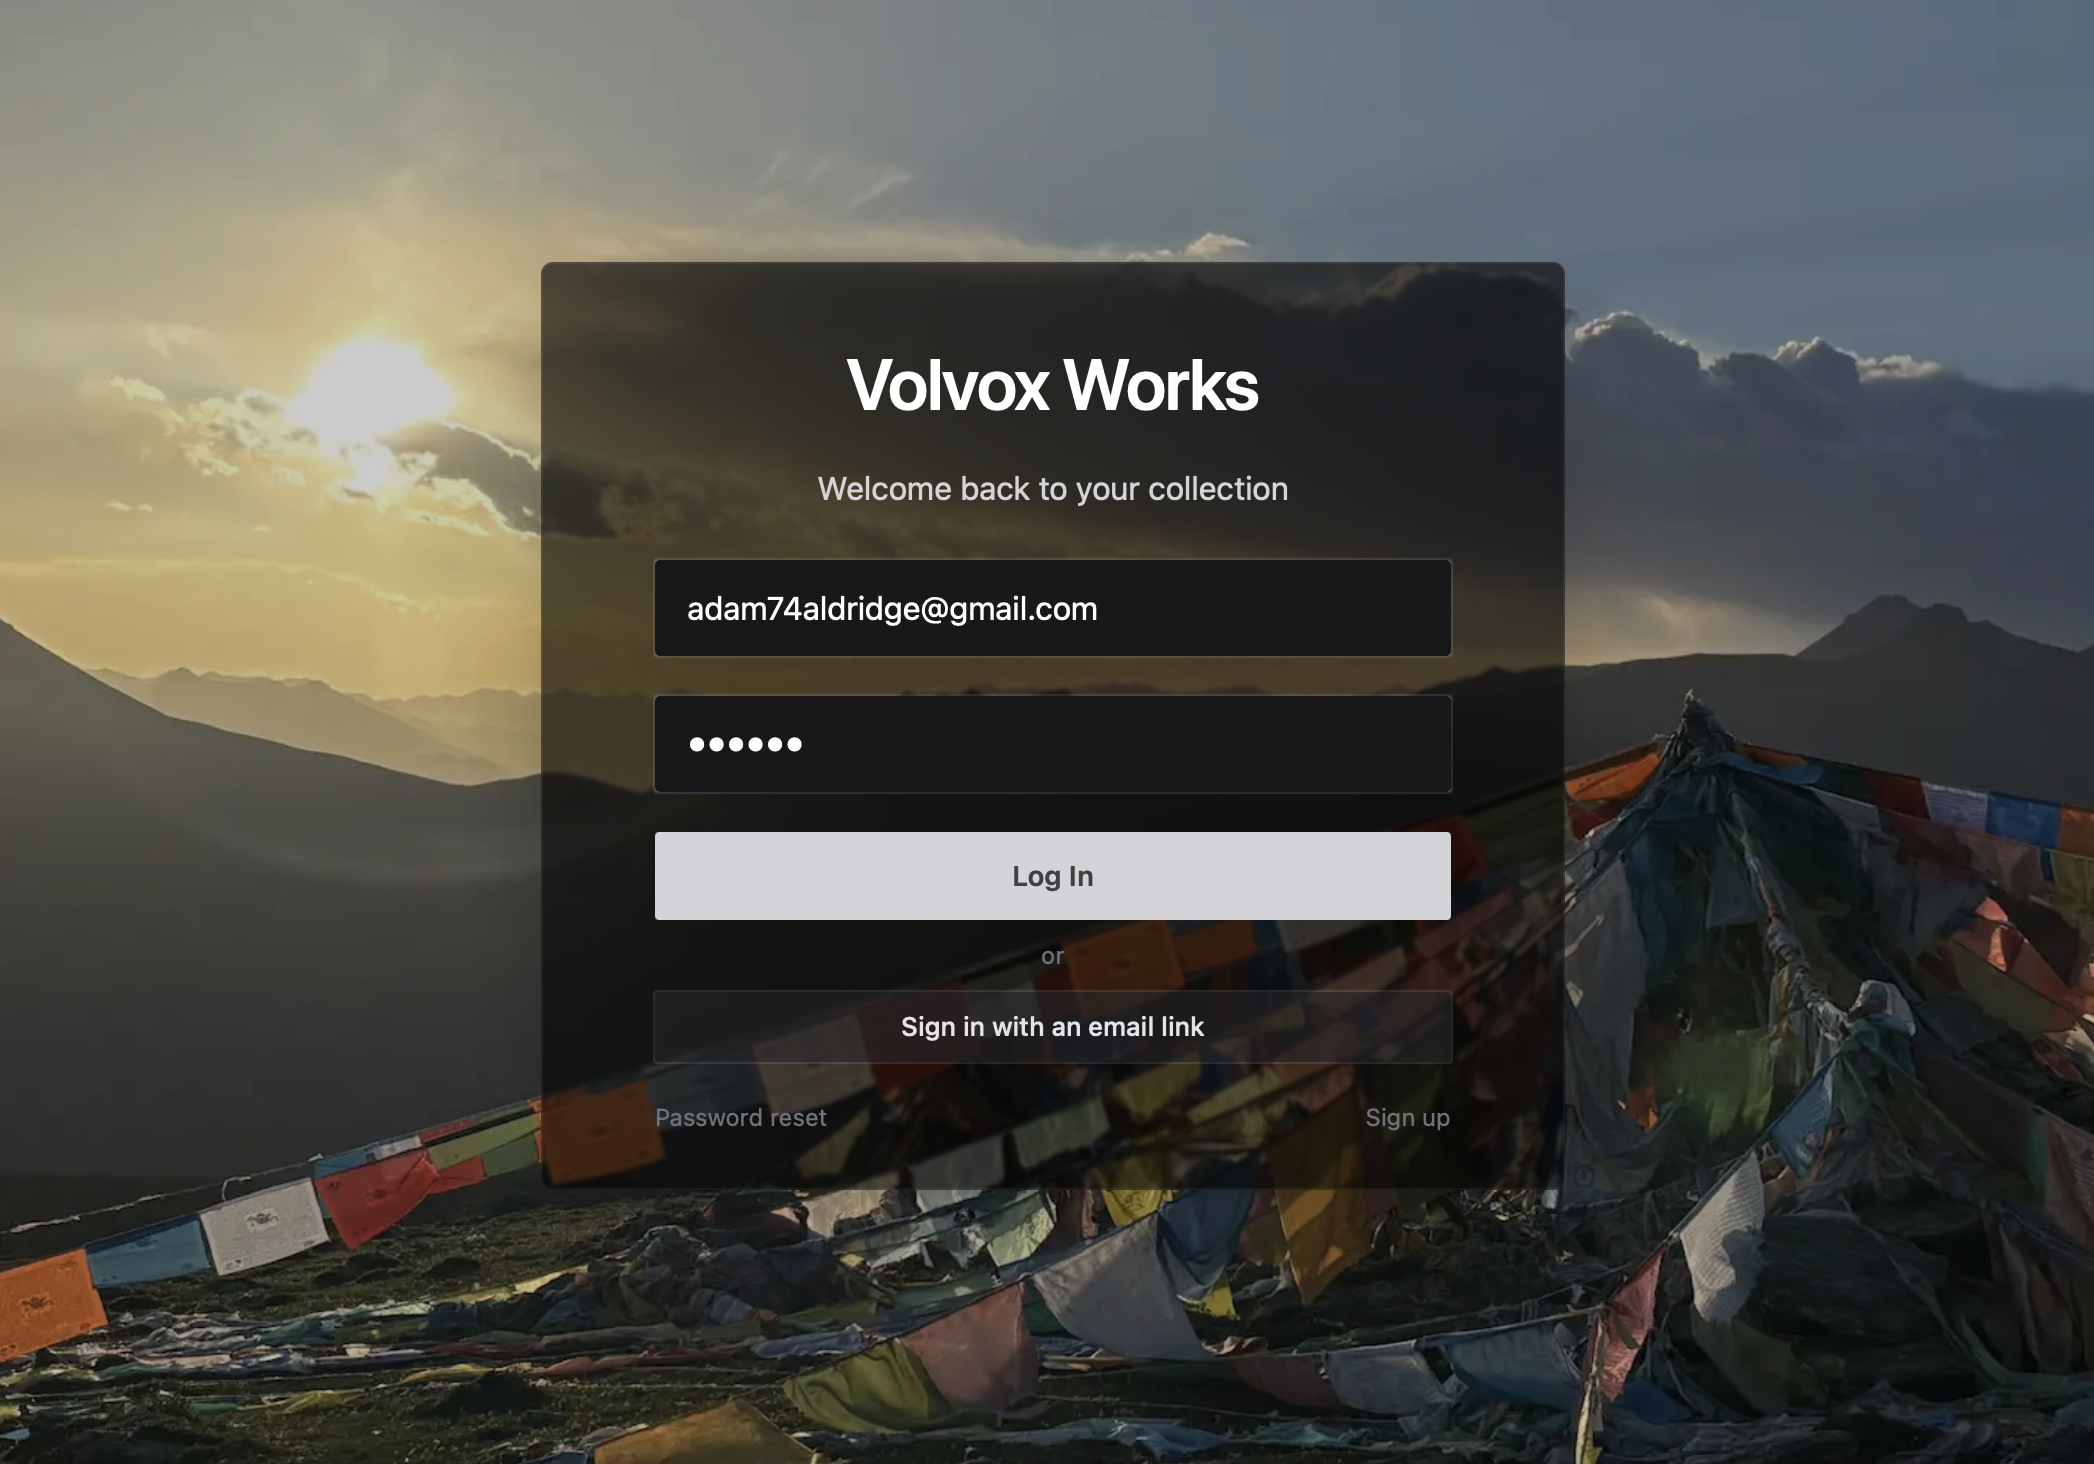
\includegraphics[width=\linewidth]{supplementary/figures/volvox-works.png}
  \captionof{figure}{The portfolio builder landing page.}
  \label{sup:fig:volvox-works}

  \vspace{0.9em}
  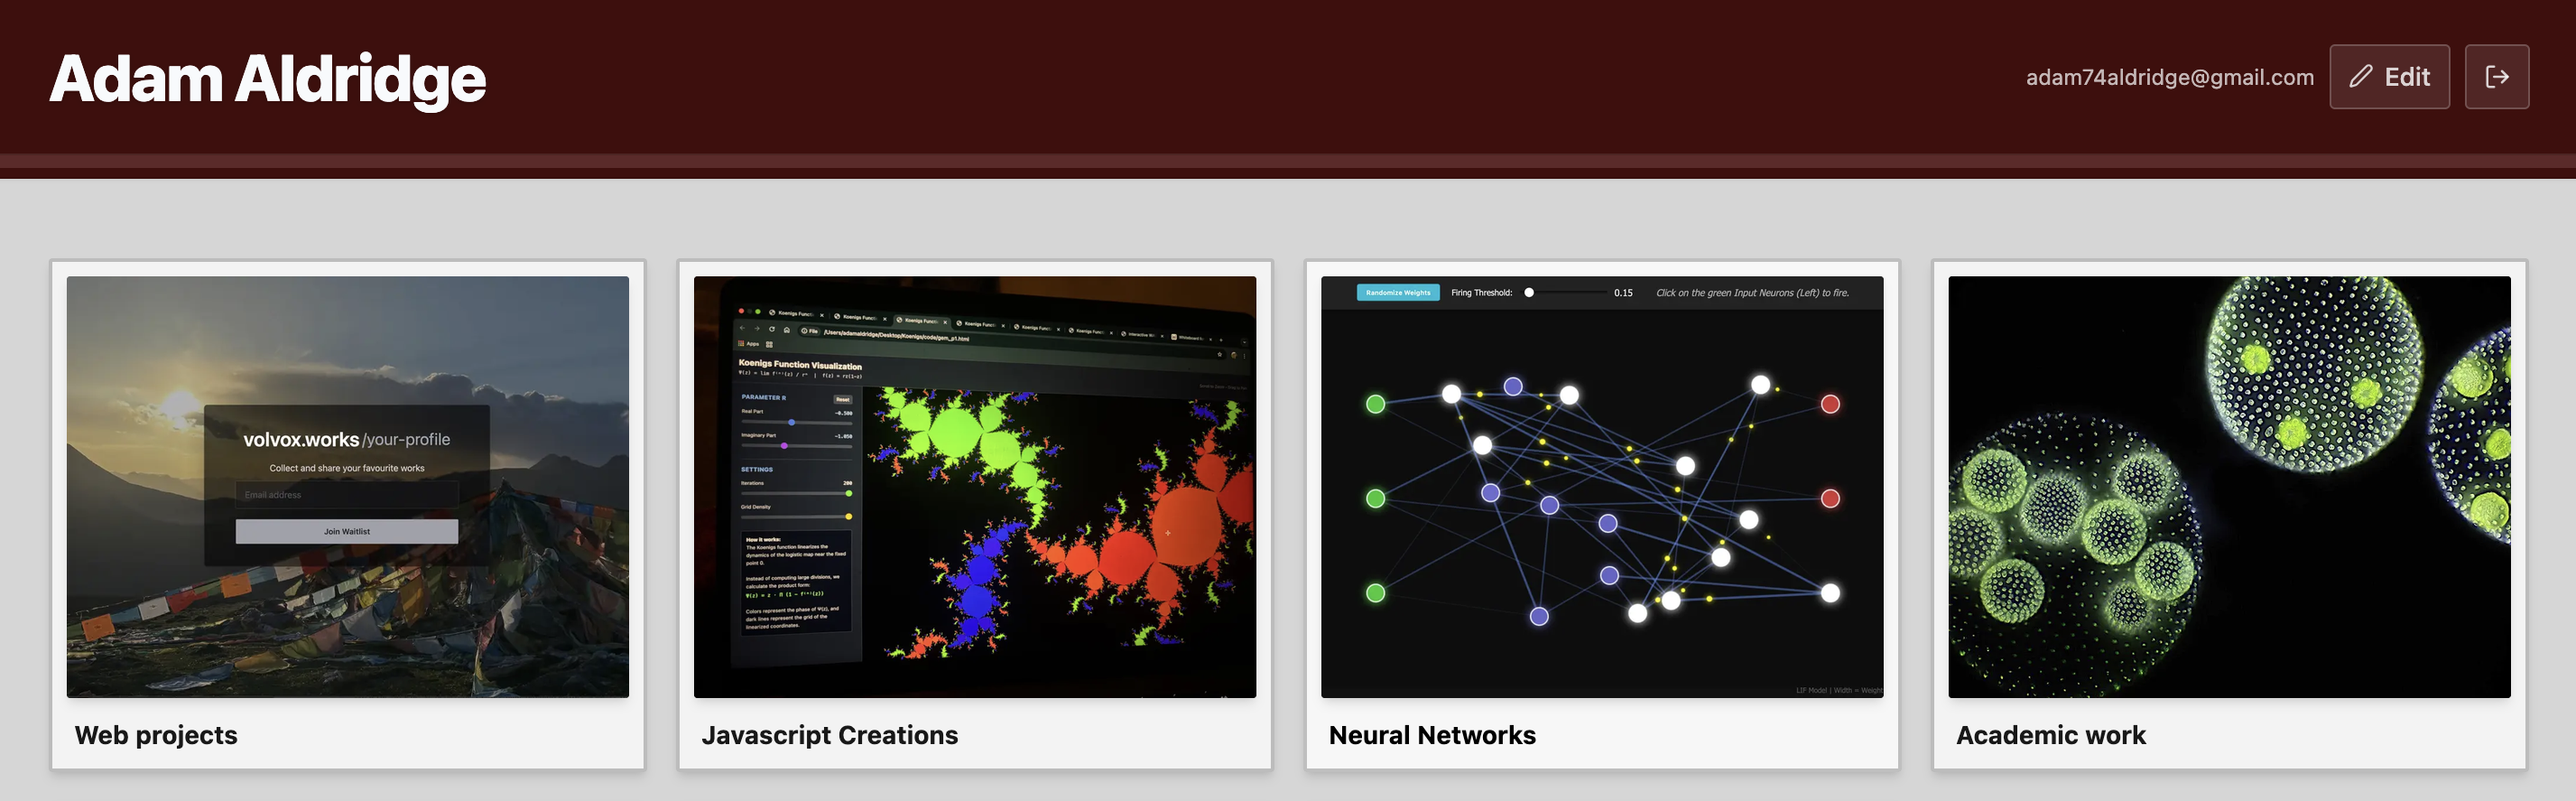
\includegraphics[width=\linewidth]{supplementary/figures/volvox-thesis.png}
  \captionof{figure}{The Volvox page collecting the full thesis content and its
    visualisers. (Links to individual applets can also be found in the relevant
    figure captions.)}
  \label{sup:fig:volvox-thesis}
\end{minipage}%
\hfill
\begin{minipage}[t]{0.59\textwidth}
  \strut\vspace{-\baselineskip}\par
  The first one is a portfolio builder at \url{\VolvoxURL}, with my personal page and the content associated with this thesis both hosted on it.

  \begin{itemize}[leftmargin=1.1em,itemsep=0.25em,topsep=0.5em,parsep=0pt]
    \item the content associated with this thesis\\ \href{\ThesisURL}{\nolinkurl{\ThesisURL}}
    \item my personal page\\ \href{\PortfolioURL}{\nolinkurl{\PortfolioURL}}
  \end{itemize}

  \medskip
  Volvox has been an ongoing project for the last couple of years. It started with a simple idea of pages and posts, and got slowly built throughout the full on-ramp of agentic coding capability. In the first month, I was learning to write Next.js React code line by line with tutorial from the codefa.st course. A few months later, I was copy and pasting blocks of code into Gemini~3 Pro to edit each component file individually. Then since the advent of OpenClaw and subsequently the new breed of agentic coding CLIs, development has been made almost trivial.
\end{minipage}

\medskip
\hrule
\medskip

% ---- App 2: Markov Side-by-Side --------------------------------------
\noindent
\begin{minipage}[t]{0.37\textwidth}
  \strut\vspace{-\baselineskip}\par
  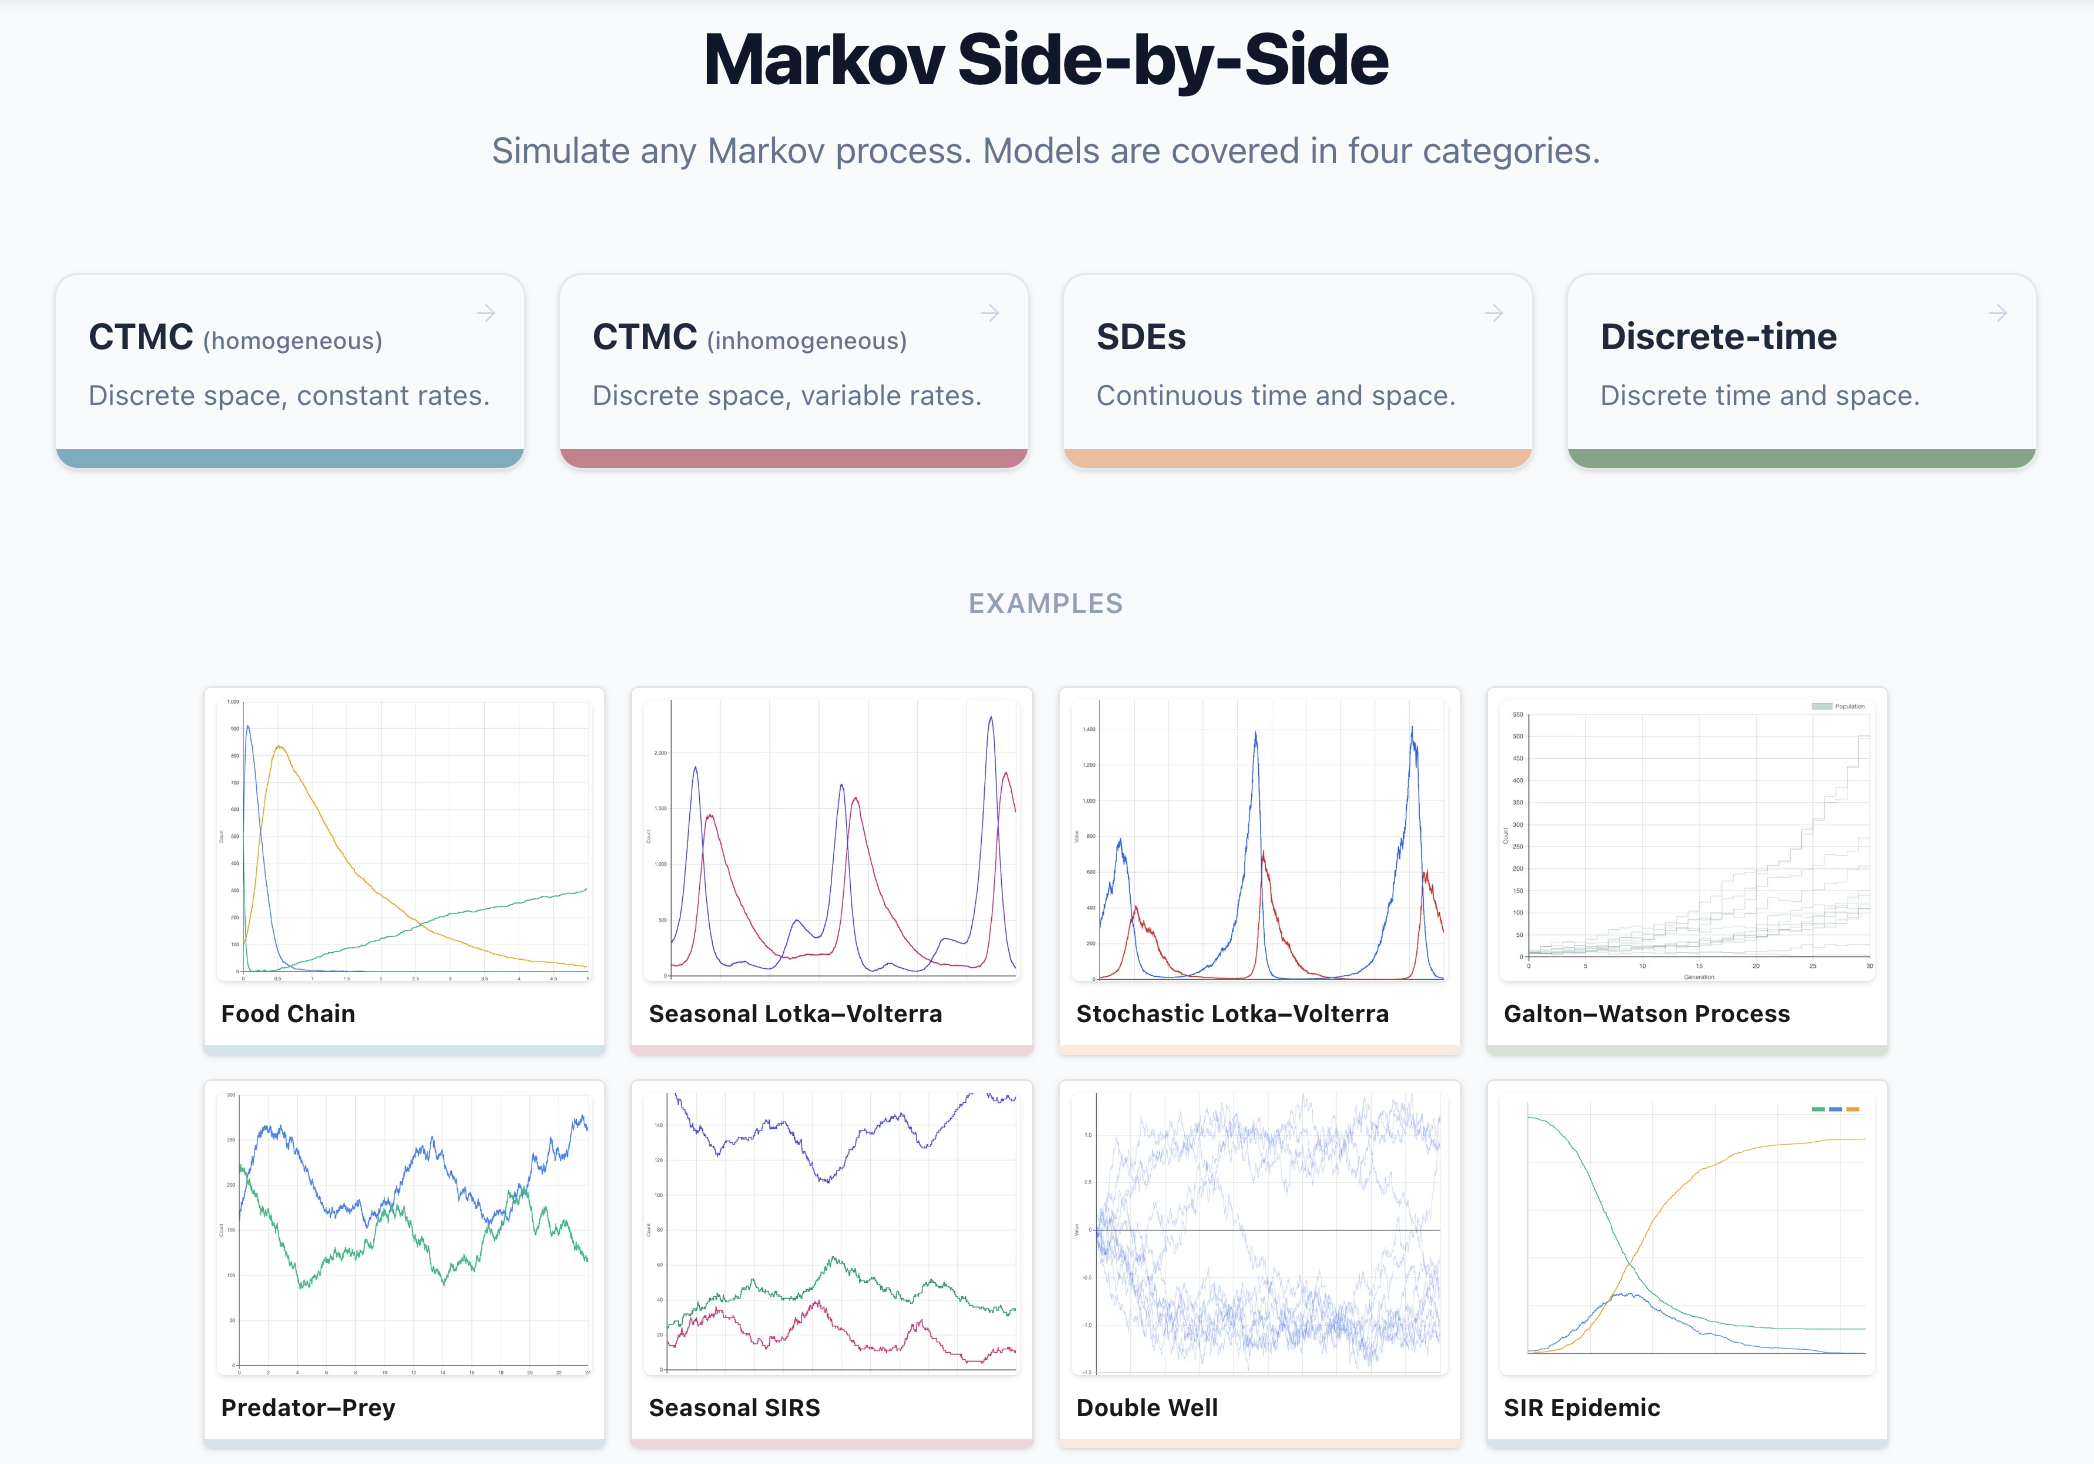
\includegraphics[width=\linewidth]{supplementary/figures/markov.png}
  \captionof{figure}{Markov Side-by-Side, where all of the Markov processes
    present in this thesis can be seen and interacted with.}
  \label{sup:fig:markov}
\end{minipage}%
\hfill
\begin{minipage}[t]{0.59\textwidth}
  \strut\vspace{-\baselineskip}\par
  The other one, Markov Side-by-Side, is a tool which lets you simulate practically any Markov process just by writing it down, and save it to your personal dashboard, which can be shared via a link.

  \begin{itemize}[leftmargin=1.1em,itemsep=0.25em,topsep=0.5em,parsep=0pt]
    \item Markov Side-by-Side\\ \href{\MarkovURL}{\nolinkurl{\MarkovURL}}
  \end{itemize}

  \medskip
  The Markov simulator works programmatically without any LLM API calls. The text inputs defining the model are encoded into a JSON config file that is read by a generalised simulation algorithm. Though, I have to say -- now it is possible to automatically generate simulations of any Markov process just with a picture of some hand written notes. But I came up with the idea for \mbox{\url{\MarkovURL}} before coding agents were able to do that.
\end{minipage}

\medskip
\hrule

\endgroup
